\documentclass[11pt]{article}
\usepackage[margin=1in]{geometry}
\usepackage{mathpazo}
\usepackage{amsmath,amssymb}
\usepackage{microtype}
\usepackage{booktabs}
\usepackage{graphicx}
\usepackage[dvipsnames]{xcolor}
\usepackage{tikz}
\usetikzlibrary{positioning,arrows.meta,calc,fit,backgrounds}
\usepackage[most]{tcolorbox}
\usepackage{enumitem}
\usepackage{listings}
\usepackage[font=small,labelfont=bf]{caption}
\usepackage{hyperref}
\hypersetup{colorlinks=true,linkcolor=MidnightBlue,citecolor=MidnightBlue,urlcolor=MidnightBlue}
\usepackage{cleveref}
\urlstyle{tt}
\def\UrlBreaks{\do\_\do/\do.}
\newcommand{\file}[1]{\nolinkurl{#1}}
\newcommand{\code}[1]{\texttt{#1}}
\newcommand{\mhh}{m_{hh}}
\newcommand{\bw}{\boldsymbol{\omega}}
\newcommand{\bp}{\boldsymbol{p}}
\newcommand{\bx}{\boldsymbol{x}}
\newcommand{\data}{\mathcal{D}}

\definecolor{trainable}{HTML}{1B6CA8}
\definecolor{physics}{HTML}{2E933C}
\definecolor{datac}{HTML}{7B4EA3}
\definecolor{warn}{HTML}{C0392B}

\newtcolorbox{keyidea}[1][]{enhanced,breakable,colback=physics!6,colframe=physics!70!black,
  fonttitle=\bfseries,title={#1},boxrule=0.6pt,arc=2pt,left=6pt,right=6pt}
\newtcolorbox{aside}[1][]{enhanced,breakable,colback=trainable!5,colframe=trainable!70!black,
  fonttitle=\bfseries,title={#1},boxrule=0.6pt,arc=2pt,left=6pt,right=6pt}
\newtcolorbox{assume}[1][]{enhanced,breakable,colback=datac!5,colframe=datac!70!black,
  fonttitle=\bfseries,title={#1},boxrule=0.6pt,arc=2pt,left=6pt,right=6pt}
\newtcolorbox{watch}[1][]{enhanced,breakable,colback=warn!5,colframe=warn!70!black,
  fonttitle=\bfseries,title={#1},boxrule=0.6pt,arc=2pt,left=6pt,right=6pt}
\setlist{itemsep=2pt,topsep=3pt}
\setlength{\emergencystretch}{3em}

\lstset{language=Python, basicstyle=\ttfamily\small, columns=fullflexible,
  keepspaces=true, commentstyle=\color{physics!70!black}\itshape,
  keywordstyle=\color{trainable!90!black}\bfseries, stringstyle=\color{datac},
  showstringspaces=false, frame=single, rulecolor=\color{gray!40},
  backgroundcolor=\color{gray!3}, xleftmargin=4pt, xrightmargin=4pt,
  aboveskip=6pt, belowskip=6pt}

\title{\textbf{A bootstrap ensemble of \texttt{HEFTNet} models}\\[4pt]
\large Plan for \texttt{heft\_train\_ensemble.ipynb} and \texttt{dihiggs/ensemble.py}\\[4pt]
\normalsize For approval before any code is written}
\date{October 30, 2026}

\begin{document}
\maketitle

\begin{abstract}
\noindent
The first Bayesian neural network run (\file{docs/bnn/bnn_run1.pdf}) gave credible
bands about 17 times narrower than the model's actual error, partly because a single
HMC chain explores a single valley of the posterior. This plan describes a
complementary, frequentist approach: train many copies of \code{HEFTNet}, each on a
\emph{bootstrap} resample of the training spectra and with its own random seed, and use
the spread of their predictions as an estimate of the standard error of the trained
network. Two ensembles are proposed: one that varies only the seed (initial weights and
batch order) on the full data, and one that also resamples the data. Together with the
BNN they separate the uncertainty due to the optimisation (which valley), the
uncertainty due to the finite training sample, and the bias that neither captures. The
work is a new notebook, \file{code/heft_train_ensemble.ipynb}, and a small new module,
\file{dihiggs/ensemble.py}. Nothing will be written until you approve; the decisions
needed are collected in \cref{sec:decisions}.
\end{abstract}

\begin{keyidea}[The proposal in brief]
\begin{enumerate}
  \item \textbf{Two ensembles} of $M = 20$ members each (\cref{tab:ensembles}):
    \code{'seeds'} (full data, different seeds) and \code{'bootstrap'} (resampled
    spectra, different seeds).
  \item \textbf{Resample whole spectra,} never individual rows: the 80 bins of a spectrum
    share $\theta$, a Monte Carlo run and the model's misfit, so they are not independent.
  \item \textbf{Each member is trained exactly as in \file{heft_train.ipynb}} (L1 loss,
    Adam, the same learning-rate steps), and saved as an ordinary run folder, so that
    \file{heft_test.ipynb} and \file{heft_export.ipynb} work with any member.
  \item \textbf{The validation spectra are chosen once,} by spectrum, and are the same for
    every member, so no copy of a training spectrum is ever used for validation.
  \item \textbf{An \code{Ensemble} class} with the same methods as \code{hmc.BNN}
    (\code{mean}, \code{std}, \code{quantiles}, \code{interval}, \code{apply}).
  \item \textbf{The test} is on the 1,000 holdout spectra: is the ensemble spread, added
    to the POWHEG noise, the size of the actual differences from POWHEG?
\end{enumerate}
\end{keyidea}

\tableofcontents

% ===========================================================================
\section{Why an ensemble}
\label{sec:why}

The BNN run showed three reasons why a single chain's band is too narrow
(\file{bnn_run1.pdf}, \S6): incomplete exploration of the valley it is in; other valleys,
in which equally good networks give different predictions where the data constrain them
weakly; and the model's own systematic error, which no spread of parameters within one
model describes. An ensemble of independently trained networks addresses the second
directly. Each training run, started from different random weights and fed batches in a
different order, ends in a different valley. Large studies have found that such
``deep ensembles'' reproduce the predictions of long, full-data HMC better than most
other approximations, precisely because they visit several valleys~\cite{izmailov2021,
wilson2020, lakshminarayanan2017}.

Resampling the training data as well, by the bootstrap~\cite{efron1993}, adds the second
source of variation that any estimator has: the training set is one finite sample, and a
different sample would give a different network.

% ===========================================================================
\section{What the ensemble estimates}
\label{sec:what}

\subsection{The frequentist view}

Think of the whole training procedure as an \emph{estimator}: it takes a training set
$D$ and a random seed $s$ and returns a function $\hat f(\bx; D, s)$. Had POWHEG been run
again, $D$ would be different; had the seed been different, the optimiser would have
ended elsewhere. So $\hat f(\bx)$ at a fixed point $\bx$ is a random variable, with a
mean and a variance. Its standard deviation is the \emph{standard error} of the trained
network at $\bx$, the frequentist counterpart of the width of a Bayesian band.

\begin{aside}[The bootstrap principle]
We have only one training set, so the distribution of $\hat f$ over training sets cannot
be observed directly. The bootstrap~\cite{efron1993} replaces the unknown population of
spectra by the sample we have: a bootstrap training set $D^*$ is made by drawing $n$
spectra \emph{with replacement} from the $n$ available. On average a bootstrap set
contains $1 - e^{-1} \approx 63\%$ of the distinct spectra, some of them more than once.
The spread of $\hat f(\bx; D^*_m, s_m)$ over $m = 1, \ldots, M$ estimates the spread of
$\hat f$ over real training sets.
\end{aside}

\subsection{Separating the two sources}
\label{sec:decomp}

The law of total variance splits the variance of $\hat f$ at $\bx$ into an optimisation
part and a data part:
\begin{equation}
  \underbrace{\operatorname{Var}_{D,s}\bigl[\hat f\bigr]}_{\text{total}}
  \;=\;
  \underbrace{\operatorname{E}_{D}\Bigl[\operatorname{Var}_{s}\bigl[\hat f \mid D\bigr]\Bigr]}_{\text{optimisation: which valley}}
  \;+\;
  \underbrace{\operatorname{Var}_{D}\Bigl[\operatorname{E}_{s}\bigl[\hat f \mid D\bigr]\Bigr]}_{\text{data: which sample}} .
  \label{eq:totvar}
\end{equation}
The two ensembles of \cref{tab:ensembles} estimate the first term and the total. The data
term is their difference, assuming the optimisation spread is about the same for a
bootstrap set as for the full set.

\begin{table}[h]
\centering\small
\begin{tabular}{lllll}
\toprule
\code{MODE} & training set of member $m$ & seed & estimates & run folder\\
\midrule
\code{'seeds'} & all training spectra & \code{SEED} $+ m$ & optimisation term & \file{runs/ENS_seeds}\\
\code{'bootstrap'} & bootstrap resample $m$ & \code{SEED} $+ m$ & total & \file{runs/ENS_bootstrap}\\
\bottomrule
\end{tabular}
\caption{The two ensembles. Member $m$ uses the same seed in both, so the two members
start from the same initial weights; only the data differ.}
\label{tab:ensembles}
\end{table}

\begin{watch}[What neither ensemble captures: the shared bias]
All members have the same architecture, the same loss and the same training schedule. If
they all miss the plateau just above threshold in the same way, they agree with each
other, and the spread stays small however many members there are. The bootstrap standard
error is an honest error bar on the \emph{estimator} $\hat f$, not on the true cross
section, unless the bias $\operatorname{E}[\hat f] - \sigma_\text{true}$ is small compared
with it. Near threshold it may not be. The test of \cref{sec:test} is designed to show
whether it is.
\end{watch}

\subsection{How many members?}

The standard deviation of $M$ draws is itself uncertain, by a relative amount of about
$1/\sqrt{2(M - 1)}$:

\begin{center}
\small
\begin{tabular}{lcccc}
\toprule
$M$ & 10 & 20 & 50 & 100\\
\midrule
relative uncertainty of the standard deviation & 24\% & 16\% & 10\% & 7\%\\
\bottomrule
\end{tabular}
\end{center}

\noindent I propose $M = 20$ per ensemble, enough to tell a factor of two in width,
which is the level of the questions we are asking. Members can be added later without
redoing the others.

% ===========================================================================
\section{Resampling spectra, not rows}
\label{sec:resample}

\begin{figure}[h]
\centering
\resizebox{\textwidth}{!}{%
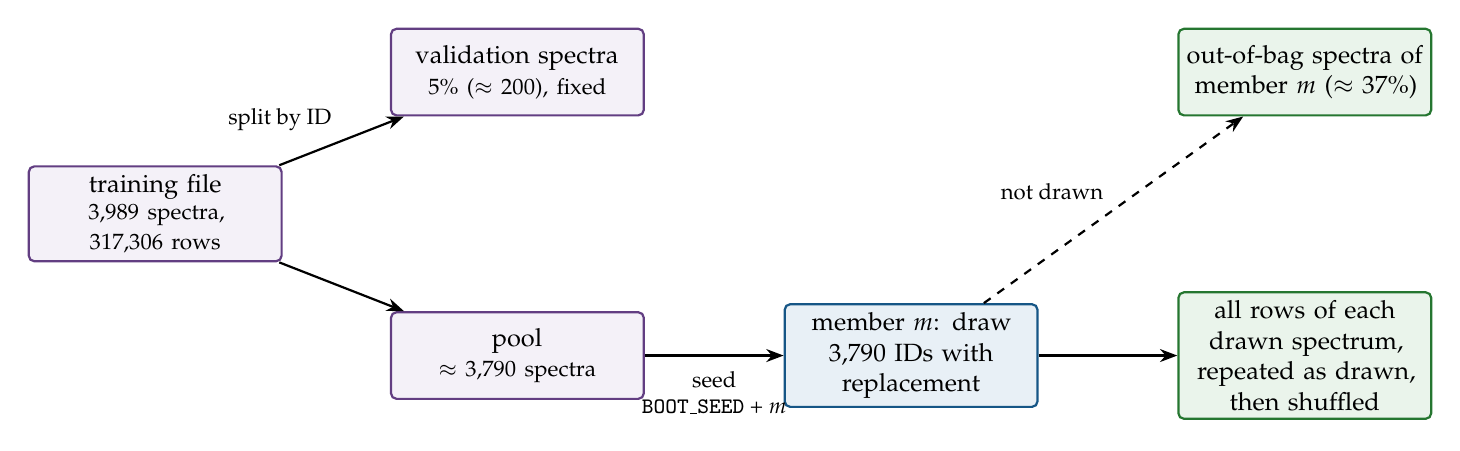
\begin{tikzpicture}[
  font=\small, >={Stealth[length=2.2mm]},
  box/.style={draw, rounded corners=2pt, thick, align=center, inner sep=3pt,
              minimum height=11mm, text width=30mm},
  dat/.style={box, fill=datac!8, draw=datac!80!black},
  nbk/.style={box, fill=trainable!10, draw=trainable!80!black},
  res/.style={box, fill=physics!10, draw=physics!80!black},
]
\node[dat] (file) at (0, 0) {training file\\\footnotesize 3,989 spectra,\\\footnotesize 317,306 rows};
\node[dat] (val)  at (4.6, 1.8) {validation spectra\\\footnotesize 5\% ($\approx$ 200), fixed};
\node[dat] (pool) at (4.6, -1.8) {pool\\\footnotesize $\approx$ 3,790 spectra};
\node[nbk] (draw) at (9.6, -1.8) {member $m$: draw 3,790 IDs with replacement};
\node[res] (rows) at (14.6, -1.8) {all rows of each drawn spectrum, repeated as drawn, then shuffled};
\node[res] (oob)  at (14.6, 1.8) {out-of-bag spectra of member $m$ ($\approx$ 37\%)};
\draw[->, thick] (file) -- node[above left, font=\footnotesize]{split by ID} (val);
\draw[->, thick] (file) -- (pool);
\draw[->, thick] (pool) -- node[below=2pt, font=\footnotesize, align=center]{seed\\\code{BOOT\_SEED} + $m$} (draw);
\draw[->, thick] (draw) -- (rows);
\draw[->, thick, dashed] (draw) -- node[above left, font=\footnotesize]{not drawn} (oob);
\end{tikzpicture}}
\caption{How the training set of one bootstrap member is formed. The validation spectra
are set aside once, for all members and both ensembles.}
\label{fig:resample}
\end{figure}

\begin{itemize}
  \item \textbf{Why spectra.} The 80 bins of a spectrum share $\theta$ and come from one
    POWHEG run, and the model's errors are correlated across them, most strongly near
    threshold. Resampling rows would treat them as 80 independent pieces of information
    and underestimate the spread, the same overconfidence that afflicts the BNN's
    likelihood. Resampling spectra is the ``block'' or ``cluster'' bootstrap.
  \item \textbf{The validation set.} \file{heft_train.ipynb} splits the training file by
    row, so a spectrum's bins are spread over training, validation and its quick-test
    rows. That is harmless for a single model, whose real test is the holdout file. In a
    bootstrap ensemble it would put copies of training spectra into validation, and the
    validation loss, which chooses the saved parameters, would be biased. So the new
    notebook sets aside 5\% of the \emph{spectra} once (seed \code{SEED}), for every
    member of both ensembles.
  \item \textbf{Shuffling.} The rows of a bootstrap set are built spectrum by spectrum, so
    they are shuffled before training. (\code{drwho}'s \code{DataLoader} reshuffles only
    after the first pass through the data.)
  \item \textbf{Bookkeeping.} Each member's folder gets \file{bootstrap_ids.csv}: the IDs
    drawn and how often. Together with \code{BOOT\_SEED} this makes every member
    reproducible and allows the \emph{out-of-bag} spectra, those a member never saw, to be
    used as a free extra test of that member.
  \item \textbf{Size.} A bootstrap set has as many spectra as the pool, so its number of
    rows, about 301,000, is close to that of the full set, and the training schedule needs
    no change.
\end{itemize}

% ===========================================================================
\section{Training the members}
\label{sec:train}

Each member is trained with the code of \file{heft_train.ipynb}, unchanged except for
the data: L1 loss (as \code{nn.L1Loss}), Adam, batch size 2,048, 200,000 iterations in
four learning-rate steps from $2 \times 10^{-3}$, parameters saved at the best
validation loss. Before member $m$ is built, \code{torch.manual\_seed(SEED + m)} and
\code{np.random.seed(SEED + m)} fix its initial weights and its batch order.

\paragraph{Run folders.} Member $m$ of an ensemble is saved in
\file{runs/ENS_<mode>/member_01/}, \file{member_02/}, \ldots, each an ordinary run folder
(\file{dihiggs_config.yaml}, \file{dihiggs_params.pth}, \file{dihiggs_losses.csv}), plus
\file{bootstrap_ids.csv} for bootstrap members. The configuration records \code{MODE},
the member number, both seeds and the training file's SHA-256. A summary file
\file{runs/ENS_<mode>/ensemble.csv} has one row per member: seeds, number of distinct
spectra, number of rows, best validation loss, out-of-bag $\chi^2/N$, training time.

\paragraph{Interruption and parallel running.} Members are trained one after another, and
a member whose parameter file and summary row already exist is skipped, so an interrupted
loop resumes where it stopped. A switch \code{MEMBERS} (e.g.\ \code{range(0, 10)}) chooses
which members a notebook trains, so that two or more copies of the notebook can train
disjoint sets of members at the same time on the 5090. \code{HEFTNet} is small; several
trainings fit on one GPU at once.

\paragraph{The real-time loss monitor.} \file{heft_train.ipynb} opens a window that plots
the losses during training. In a loop over 20 members that would open 20 windows, so the
ensemble notebook writes the loss files without starting the window
(\code{monitor.start()} is not called); progress is printed instead.

\paragraph{Cost.} About 42 minutes per member on a CPU; on the 5090 I expect a few
minutes, but the notebook will time the first member and print an estimate for the rest.
The \code{N\_ITERATIONS} switch allows shorter members for a first trial.

% ===========================================================================
\section{The module \texttt{dihiggs/ensemble.py}}
\label{sec:module}

A class \code{Ensemble} with the same interface as \code{hmc.BNN}, so that analysis code
can use either:

\begin{lstlisting}
from dihiggs import ensemble
from dihiggs import heftnet as NN

ens = ensemble.Ensemble(NN.HEFTNet, 'runs/ENS_bootstrap')  # every member_*/
mu  = ens.mean(x)                  # ensemble mean, one value per row of x
sd  = ens.std(x)                   # spread of the members (the standard error)
lo, hi = ens.interval(x, cl=0.68)  # central 68% of the members
A   = ens.apply(lambda m, x: m.coeffs(x), xs)   # a_i(m_hh) for every member
\end{lstlisting}

\noindent It reads \file{member_*/dihiggs_params.pth} by default (any file pattern can be
given), and also provides \code{summary()}, the contents of \file{ensemble.csv}. Like
\file{hmc.py}, it imports nothing from \code{dihiggs}, so it can move to \code{drwho}.

\begin{aside}[Why not reuse \texttt{hmc.BNN} directly?]
\code{BNN} already averages over a list of parameter files, and an ensemble needs the same
arithmetic. The tidy design is a common base class (an ensemble of parameter files) of
which \code{BNN} is a special case that also reads the noise scales. I propose to write
\code{Ensemble} as that base class now, and to make \code{BNN} a subclass of it when both
modules move to \code{drwho}, so that \file{hmc.py}, which works and has been checked, is
not changed now (\cref{sec:decisions}).
\end{aside}

% ===========================================================================
\section{The notebook \texttt{heft\_train\_ensemble.ipynb}}
\label{sec:notebook}

In the style of \file{heft_train.ipynb} (header, Colab cell with \code{USE\_DRIVE},
imports, device, data with its SHA-256), then:

\begin{enumerate}
  \item \textbf{Introduction} (markdown): the estimator view, the bootstrap, the
    decomposition (\ref{eq:totvar}), and why spectra are resampled.
  \item \textbf{Switches:} \code{MODE = 'bootstrap'} or \code{'seeds'};
    \code{N\_MEMBERS = 20}; \code{MEMBERS = range(N\_MEMBERS)}; \code{SEED = 42};
    \code{BOOT\_SEED = 1000}; \code{VAL\_FRACTION = 0.05};
    \code{N\_ITERATIONS = 200\_000}. \code{DIRNAME} = \file{ENS_<mode>}.
  \item \textbf{The split by spectrum:} validation IDs and the pool, printed with a
    fingerprint of the validation IDs (as \file{heft_prepare_data} does for the holdout).
  \item \textbf{One member's data:} a function returning the shuffled rows of member $m$
    and its table of drawn IDs.
  \item \textbf{One member's training:} a function that builds the configuration, model,
    optimiser, scheduler and monitor, trains, and appends the summary row; the training
    loop is that of \file{heft_train.ipynb}.
  \item \textbf{The loop} over \code{MEMBERS}, skipping finished members.
  \item \textbf{Results on the holdout spectra} (\cref{sec:test}): the ensemble mean
    against POWHEG; spectra with ensemble bands; the spread against $\mhh$; the pull test;
    and, when both ensembles exist, the decomposition (\ref{eq:totvar}) against $\mhh$, and
    the comparison with the BNN run if there is one.
\end{enumerate}

% ===========================================================================
\section{The test: is the spread the size of the error?}
\label{sec:test}

On the 1,000 holdout spectra, at every bin $k$ with POWHEG value $t_k$, POWHEG noise
$\sigma_k$ (as in \file{heft_test.ipynb}), ensemble mean $\bar f_k$ and ensemble standard
deviation $s_k$, form the pull
\begin{equation}
  z_k = \frac{t_k - \bar f_k}{\sqrt{\sigma_k^2 + s_k^2}} .
  \label{eq:pull}
\end{equation}
If the ensemble spread describes the model's error, and the error and the POWHEG noise
are independent, $z_k$ has mean 0 and standard deviation 1, and $|z_k| < 2$ for about
95\% of bins. If the spread is too small, the standard deviation of $z$ is larger than 1.
The same pull, with $s_k$ the posterior standard deviation, is computed for the BNN, so all
three are compared on one scale.

\begin{center}
\small
\begin{tabular}{p{0.42\textwidth}p{0.50\textwidth}}
\toprule
quantity & reported\\
\midrule
accuracy of the ensemble mean & median $\chi^2/N$; fractions above 2 and 5; mean $\chi^2$ per
  bin at 255--555 GeV and above; against the single members and the L1 model\\
width & $s_k/\sigma_k$: median, distribution, against $\mhh$\\
calibration & standard deviation of $z$; fraction $|z| < 2$; both against $\mhh$\\
decomposition & optimisation and data terms of (\ref{eq:totvar}) against $\mhh$\\
out-of-bag (bootstrap only) & each member's $\chi^2/N$ on the spectra it did not see\\
\bottomrule
\end{tabular}
\end{center}

\paragraph{What counts as success.}
\begin{enumerate}
  \item The ensemble mean is at least as accurate as a single L1 model, as averaging over
    members usually makes it.
  \item The spread is \emph{informative}: larger where the model is known to be weak
    (near threshold) than elsewhere.
  \item The standard deviation of $z$ is close to 1 above about 555 GeV. Near threshold I
    expect it to exceed 1, because of the shared bias; how much it exceeds 1 measures that
    bias, which is itself a useful number.
\end{enumerate}

% ===========================================================================
\section{Links with the BNN}

\begin{itemize}
  \item \textbf{Starting points for several HMC chains.} The members of the
    \code{'seeds'} ensemble lie in different valleys. Starting four BNN chains from four of
    them makes $\hat R$ across chains a real test for several valleys, which it is not when
    every chain starts from the same L1 model. This needs a small option in
    \file{heft_train_bnn.ipynb}, \code{START\_FROM}, a list of parameter files, one per
    chain, to be added after this plan.
  \item \textbf{A common yardstick.} The pull (\ref{eq:pull}) puts the BNN band, the two
    ensemble spreads and the POWHEG noise on one scale.
\end{itemize}

% ===========================================================================
\section{Not in this plan}
\begin{itemize}
  \item No change to \file{heft_train.ipynb}, \file{heft_test.ipynb}, \file{hmc.py} or the
    data files.
  \item The \code{START\_FROM} option of the BNN notebook (above), and the tempered
    likelihood discussed on October 30, are separate steps.
  \item Bootstrap confidence intervals more refined than the spread (percentile, BCa) are
    left out: with $M = 20$ only the standard deviation is well determined.
  \item Nothing is committed to git.
\end{itemize}

% ===========================================================================
\section{Decisions for you}
\label{sec:decisions}

\begin{keyidea}[Decisions before I proceed]
\begin{enumerate}
  \item \textbf{Two ensembles,} \code{'seeds'} and \code{'bootstrap'}, $M = 20$ each.
    Agreed, or start with 10?
  \item \textbf{Validation by spectrum,} 5\% of the training spectra, fixed for all
    members. Agreed?
  \item \textbf{The training recipe} of \file{heft_train.ipynb}, unchanged (L1, 200,000
    iterations). Agreed?
  \item \textbf{No real-time monitor window} during ensemble training; printed progress
    instead. Agreed?
  \item \textbf{\code{Ensemble} as a new module,} \file{dihiggs/ensemble.py}, leaving
    \file{hmc.py} unchanged for now. Agreed?
  \item \textbf{Folder names:} \file{runs/ENS_seeds/member_01/}, \ldots. Acceptable?
  \item \textbf{Location of this document:} \file{docs/ensemble/ensemble_plan.pdf}?
\end{enumerate}
\end{keyidea}

% ===========================================================================
\begin{thebibliography}{9}
\bibitem{efron1993} B.~Efron and R.~J.~Tibshirani, \emph{An Introduction to the
  Bootstrap}, Chapman \& Hall/CRC (1993).
\bibitem{lakshminarayanan2017} B.~Lakshminarayanan, A.~Pritzel and C.~Blundell, ``Simple
  and scalable predictive uncertainty estimation using deep ensembles'', NeurIPS 2017,
  arXiv:1612.01474.
\bibitem{wilson2020} A.~G.~Wilson and P.~Izmailov, ``Bayesian deep learning and a
  probabilistic perspective of generalization'', NeurIPS 2020, arXiv:2002.08791.
\bibitem{izmailov2021} P.~Izmailov, S.~Vikram, M.~D.~Hoffman and A.~G.~Wilson, ``What are
  Bayesian neural network posteriors really like?'', ICML 2021, arXiv:2104.14421.
\end{thebibliography}

\end{document}
